% !TeX root = main.tex

\documentclass[10pt,conference]{IEEEtran}
\IEEEoverridecommandlockouts
% The preceding line is only needed to identify funding in the first footnote. If that is unneeded, please comment it out.

\usepackage{cite}
\usepackage{algpseudocode}
\usepackage[figure,linesnumbered,inoutnumbered,longend]{algorithm2e}
\usepackage{rotating,tabularx}
\usepackage{listings}
\usepackage{lstautogobble}
\usepackage{textcomp}
\usepackage{float} 
\usepackage{multicol}
\usepackage{caption}
\usepackage{adjustbox}
\usepackage{subcaption}
\usepackage{multicol}
\usepackage{pdfpages}								%Pdf manipulations.
\usepackage{setspace}
\usepackage{verbatim}
\usepackage{amsmath}
\usepackage{amssymb}
\usepackage{xfrac}
\usepackage{bm}
\usepackage[square,numbers]{natbib}
%\usepackage[colorlinks,citecolor=blue]{hyperref}
\usepackage[colorlinks = true,
            linkcolor = blue,
            urlcolor  = blue,
            citecolor = blue,
            anchorcolor = blue]{hyperref}
\usepackage{color}
%\usepackage{acronym}
\RequirePackage[printonlyused,withpage]{acronym}
\usepackage{makecell}
\setlength{\parskip}{0.05in}
%\pdfminorversion=7
\newcounter{figCount}%      This is an internal counter to track how many figures
\setcounter{figCount}{1}%   We will start at 1 due to how stepping it works.

\newcommand{\addFigure}[3][\Alph{figCount}]{%   Command to manually add a figure
    \parbox{#2\textwidth}{\centering #1 \\ \includegraphics[width=#2\textwidth]{#3}}
    \stepcounter{figCount}
    }

\newenvironment{multiFigure}% Environment that mimicks figure type environment,
%                               Except it doesn't float around and it resets figCount.
    {% Begin Environment Code
        \setcounter{figCount}{1}
        \minipage\textwidth
    }
    {% End Environment Co
        \endminipage
    }

\makeatletter
\def\input@path{{../rpt_common}}
%or: \def\input@path{{/path/to/folder/}{/path/to/other/folder/}}
\makeatother

\def\BibTeX{{\rm B\kern-.05em{\sc i\kern-.025em b}\kern-.08em
    T\kern-.1667em\lower.7ex\hbox{E}\kern-.125emX}}

\SetAlFnt{\footnotesize}
\SetAlCapFnt{\small}
\SetAlCapNameFnt{\small}

%% JMB MY STUFF %%%%%%%%%%%%%%%%%%%%%%%%%%%%%%%%%%%%%%%%%%%%%%%%%%%%%%%%%%%%%
\definecolor{Abstractcolor}{rgb}{0,0.6,0}
\definecolor{Commentcolor}{rgb}{0.74,0.11,0.16}
\definecolor{Objectcolor}{rgb}{0.6,0.0,0.4}
\definecolor{mygreen}{rgb}{0,0.6,0}
\definecolor{mygray}{rgb}{0.5,0.5,0.5}
\definecolor{mymauve}{rgb}{0.58,0,0.82}
\definecolor{mybk}{rgb}{0.95,0.95,0.95}

\newcommand{\ctxt}[1]{\textcolor{Commentcolor}{\\ \small QUOTE: #1 :ENDQUOTE \\}}
\newcommand{\jorg}[1]{\textcolor{red}{#1}}
\newcommand{\ncite}[1]{\textcolor{red}{CITE:#1}}
\newcommand{\todo}[1]{\textcolor{blue}{TODO:#1}}
\newcommand{\intendThe }[1]{\textcolor{blue}{GOAL:#1}}
\newcommand{\dens}{\mathfrak{m}}
% Format comments in algorithm
\newcommand\mycommfont[1]{\footnotesize\ttfamily\textcolor{blue}{#1}}
  
\newcommand{\algo}[1]{Fig. #1}
\newcommand{\algn}[2]{Fig. #1, line #2}
\newcommand{\Algo}[1]{Fig. #1}
\newcommand{\Algn}[2]{Fig #1, line #2}
\newcommand{\figo}[1]{fig. \ref{fig:#1}}
\newcommand{\Figo}[1]{Fig. \ref{fig:#1}}
\newcommand{\figob}[2]{fig. \ref{fig:#1}-(#2)}
\newcommand{\Figob}[2]{Fig. \ref{fig:#1}-(#2)}
\newcommand{\tigo}[1]{table \ref{tab:#1}}
\newcommand{\Tigo}[1]{Table \ref{tab:#1}}


\newcommand{\app}{\textbf{\textit{rccdApp}}}
\newcommand{\ver}{\textit{\textbf{verApp}}}
\newcommand{\gen}{\textit{\textbf{genApp}}}
\newcommand{\mmrr}{\textit{\textbf{mmrr}}}
\newcommand{\marr}{\textit{\textbf{marr}}}
\newcommand{\arr}{\textit{\textbf{arr}}}
\newcommand{\garr}{\textit{\textbf{garr}}}
\newcommand{\carr}{\textit{\textbf{carr}}}
\newcommand{\mcpt}{\textit{\textbf{mcpt}}}
\newcommand{\mgpt}{\textit{\textbf{mgpt}}}
\newcommand{\mtpt}{\textit{\textbf{mtpt}}}
\newcommand{\tarr}{\textit{\textbf{tarr}}}
\newcommand{\gpuarr}{\textit{\textbf{gpuarr}}}
\newcommand{\mat}{\textit{\textbf{matApp}}}
\newcommand{\rtrr}{\textit{\textbf{rtrr}}}
\newcommand{\tspf}{\textit{\textbf{tspf}}}
\newcommand{\tfps}{\textit{\textbf{tfps}}}
\newcommand{\gfps}{\textit{\textbf{gpufps}}}
\newcommand{\cpuarr}{\textit{\textbf{cpuarr}}}
\newcommand{\quan}{$\bm{l_q}$}
\newcommand{\pdens}{$\bm{D}$}
\newcommand{\vol}{$\bm{l_c}$}
\newcommand{\maxp}{$\bm{max_p}$}
\newcommand{\cdens}{$\bm{F}$}
\newcommand{\ccdens}{$\bm{f}$}
\newcommand{\slen}{$\bm{L_{s}}$}
\newcommand{\radius}{$\bm{R}$}
\newcommand{\bestTime}{27 fps}
\newcommand{\bestNumberParts}{4,260,864}
\SetKwComment{Comt}{$\triangleright$\ }{}

\usepackage{nicematrix}
\bibliographystyle{../bst/IEEEtranSNLink}


\usepackage{verbatim}		
\usepackage{listings}			


\lstdefinestyle{gpucode}{
language=C,
keywordstyle=\color{blue},
commentstyle=\color{Commentcolor},
stringstyle=\color{darkgray},
numbers=left,
stepnumber=1,
numbersep=5pt,
numberstyle=\tiny,
breaklines=true,
breakautoindent=true,
breakatwhitespace=false,
frame=single,	          
title=\lstname,     
postbreak=\space,
tabsize=4,
basicstyle=\tiny, %\ttfamily\scriptsize,
showspaces=false,
showstringspaces=false,
extendedchars=true,
backgroundcolor=\color{white},
 morekeywords=[2]{layout},
 morekeywords=[3]{binding},
 morekeywords=[4]{uniform},
 morekeywords=[5]{location},
 morekeywords=[6]{in},
 morekeywords=[7]{out},
 morekeywords=[8]{vec3},
 morekeywords=[9]{vec2},
 morekeywords=[10]{vec4},
 morekeywords=[11]{mat4},
 morekeywords=[12]{gl_Position},
 morekeywords=[13]{version},
 morekeywords=[14]{float},
 morekeywords=[15]{Particle},
 morekeywords=[16]{inout},
 morekeywords=[17]{uint},
 morekeywords=[18]{WIDTH},
 keywordstyle = [2]\color{blue},
 keywordstyle = [3]\color{blue},
 keywordstyle = [4]\color{blue},
 keywordstyle = [5]\color{blue},
 keywordstyle = [6]\color{blue},
 keywordstyle = [7]\color{blue},
 keywordstyle = [8]\color{violet},
 keywordstyle = [9]\color{violet},
 keywordstyle = [10]\color{violet},
 keywordstyle = [11]\color{violet},
 keywordstyle = [12]\color{violet},
 keywordstyle = [13]\color{green},
 keywordstyle = [14]\color{violet},
 keywordstyle = [15]\color{ForestGreen},
 keywordstyle = [16]\color{blue},
 keywordstyle = [17]\color{blue},
 keywordstyle = [18]\color{mymauve}
 }



\lstdefinestyle{ccode}{
  backgroundcolor=\color{white},   % choose the background color; you must add \usepackage{color} or \usepackage{xcolor}
  basicstyle=\footnotesize,        % the size of the fonts that are used for the code
  breakatwhitespace=false,         % sets if automatic breaks should only happen at whitespace
  breaklines=true,                 % sets automatic line breaking
  captionpos=b,                    % sets the caption-position to bottom
  commentstyle=\color{mygreen},    % comment style
  deletekeywords={...},            % if you want to delete keywords from the given language
  escapeinside={\%*}{*)},          % if you want to add LaTeX within your code
  extendedchars=true,              % lets you use non-ASCII characters; for 8-bits encodings only, does not work with UTF-8
  frame=single,	                   % adds a frame around the code
  keepspaces=true,                 % keeps spaces in text, useful for keeping indentation of code (possibly needs columns=flexible)
  keywordstyle=\color{blue},       % keyword style
  language=Octave,                 % the language of the code
  otherkeywords={*,...},            % if you want to add more keywords to the set
  numbers=left,                    % where to put the line-numbers; possible values are (none, left, right)
  numbersep=5pt,                   % how far the line-numbers are from the code
  numberstyle=\tiny\color{mygray}, % the style that is used for the line-numbers
  rulecolor=\color{black},         % if not set, the frame-color may be changed on line-breaks within not-black text (e.g. comments (green here))
  showspaces=false,                % show spaces everywhere adding particular underscores; it overrides 'showstringspaces'
  showstringspaces=false,          % underline spaces within strings only
  showtabs=false,                  % show tabs within strings adding particular underscores
  stepnumber=2,                    % the step between two line-numbers. If it's 1, each line will be numbered
  stringstyle=\color{mymauve},     % string literal style
  tabsize=2,	                   % sets default tabsize to 2 spaces
  title=\lstname                   % show the filename of files included with \lstinputlisting; also try caption instead of title
}
\include{../code/code_tst.tex}

\lstnewenvironment{queryl}[1][] 
 {\lstset{frame=shadowbox,escapechar=`,linewidth=8cm, #1}}
 {}

\def\StripPrefix#1>{}
\def\isOverleaf{\fi
	\def\overleafJobname{output}% overleaf defaults to 'output' as \jobname
	\edef\overleafJobname{\expandafter\StripPrefix\meaning\overleafJobname}%
	\edef\job{\jobname}%
	\ifx\job\overleafJobname
}
%\if\isOverleaf
%\bibliographystyle{/bst/IEEEtranSNLink}
 % References. First 				
%\else
\bibliographystyle{../bst/IEEEtranSNLink}   % References. First 
%\fi

\setlength{\textfloatsep}{0.1cm}

\begin{document}
\pagenumbering{arabic}
%\includepdf[pages={1-2}]{../orig/CoverSheet.pdf}
\title{Status Report \\ Rigid Fiber using (RCCD) rounded cell collision detection and regions of interest.}


\author{
\IEEEauthorblockN{Jackie Bell}
\IEEEauthorblockA{\textit{Department of Mechanical} \\
\textit{and Aerospace Engineering} \\
\textit{University of Florida}\\
Gainesville Florida,United States \\
0009-0001-4291-2230}


}
\maketitle

\pagestyle{plain}
\begin{abstract}
  
\end{abstract}

\begin{IEEEkeywords}
particle system, image space, collision detection, nearest neighbor, region of interest, GPU, GPGPU.
\end{IEEEkeywords}

% !TeX root = main.tex

\section{Overview} \label{ovr}

The way I approach any project is to break the system up into small parts then analyze and debug those parts in Matlab. This divide and conquer gives me a greater understanding of the parts and increases the chances of code working immediately once incorporated into the glsl. I will make the code available as I progress so that those involved can progress along with me. This will also provide a learning path for anyone joining the project at a later date. I don't want to become indispensable. The approach at every stage is tentative and I will await review before continuing.

\section{Rigid Fiber P001} \label{p001}

The first step in this project is to determine the structure of a rod. 
\Figo{RodStructure} shows a single rod containing 5 particles. 
\begin{figure}[H]
\centering
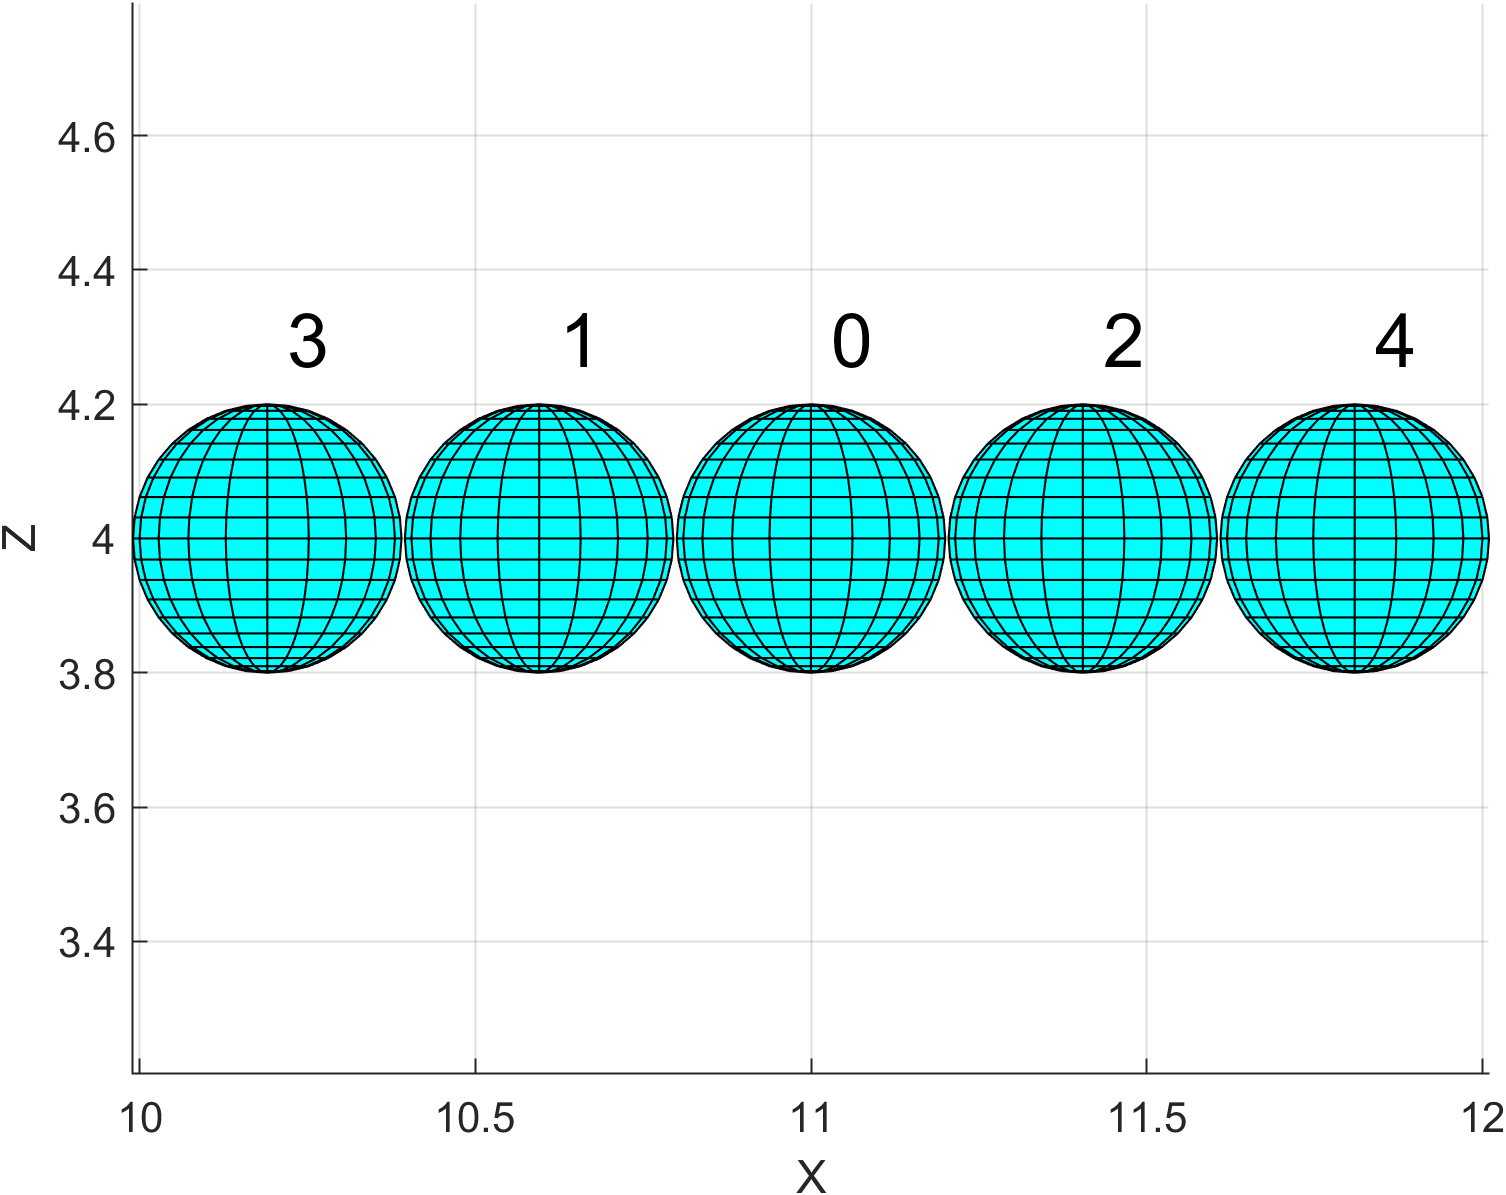
\includegraphics[width=3.40in]{../../../../RCCDRigidFiber/images//RodStructure1.png}
\captionof{figure}[Single Ros.]{\textit{A single rod showing the structure}}
\label{fig:RodStructure}
\end{figure}


Each rod has a \textit{rod number}, \texttt{rnum}, an \textit{in rod} particle, or \textit{member}, number \texttt{inum}, and the number of particles that constitute the rod, \texttt{N}. Each particle continues to have a unique particle ID, \texttt{pnum}.
 
The tentative rules are:
\begin{itemize}
\item The rod particles do not overlap since they are part of the same structure and this would waste collision detection for parts we know are already bonded.
\item The central particle has its origin at the center of mass and \texttt{inum} is equal to 0.
\item The particles to the left of the central particle have even numbered \texttt{inum}.
\item The particles to the right of the central particle have odd numbered \texttt{inum}.
\item This means that the number of particles that make up a rod, \texttt{N}, are always odd.
\item The particles will not overlap and we can use a three dimensional momentum equation to 'impulse' the particles back to their boundaries (this can be complicated since one should not use the square root or modulus on a GPU).
\end{itemize}

This will require two compute phases. The first compute will be threaded by particle and calculates individual particle collisions and reactions (by processing the \textit{potentially colliding set},(PCS) constructed by the graphics phase. The next compute phase will will be threaded by rod number and will calculate the reaction of the whole rod due to collision reactions of its member particles. The efficienty here is that once the collisions are processed in the first compute run, the collisions are stored in memory and we do not need to do it again. 

The change in position of the rod is calculated in the vertex phase. This is due to the fact that we cannot change the position of particle in the compute phase as this would corrupt the collision queries.




%% !TeX root = main.tex
\newpage
\clearpage
\section{Figures} \label{figs}
\onecolumn



% !TeX root = main.tex
\newpage
\clearpage

%\if\isOverleaf
%\bibliography{/bib/ReferencesWithdoi}
 % References. First 				
%\else
%\bibliography{../bib/Referencesdoi}
%\fi


%\input{ReviewNeeded}
%\input{todo}


\end{document}
